%% Manuscript prepared with the Copernicus Publications LaTeX package (v7.16).
%% Build: tectonic -X compile manuscript.tex   (or latexmk -pdf manuscript.tex with pdfLaTeX)
%% Journal: The Cryosphere (tc). Switch to Climate of the Past with [cp, manuscript].
\documentclass[tc, manuscript]{copernicus}

%% Page size. The class adds a 3 mm printer's bleed around the 210 x 240 mm manuscript page and, under
%% pdfLaTeX, hides it with a /CropBox. XeTeX (Tectonic) ignores that box, so the bleed is removed here to get
%% the same 210 x 240 mm page. For printing, manuscript_A4.tex defines \afour and gets an A4 page with
%% a taller text block (whole lines added).
\hoffset=-1in
\voffset=-1in
\paperwidth=210mm
\ifdefined\afour
  \paperheight=297mm
  \dimen0=57mm
  \count0=\dimen0
  \divide\count0 by \baselineskip
  \advance\textheight by \count0\baselineskip
\else
  \paperheight=240mm
\fi

\usetikzlibrary{positioning,arrows.meta,fit,backgrounds,calc}

\newcommand{\degC}{\unit{^{\circ}C}}
\newcommand{\myr}{\unit{m\,yr^{-1}}}
\newcommand{\mwe}{\unit{m\,w.e.\,yr^{-1}}}
\newcommand{\ddfunit}{\unit{mm\,w.e.\,K^{-1}\,d^{-1}}}
\newcommand{\Aunit}{\unit{MPa^{-3}\,yr^{-1}}}
\newcommand{\taur}{\tau_\mathrm{ref}}
\newcommand{\ubar}{\bar{\vec{u}}}
\newcommand{\sg}{\operatorname{sg}}

\begin{document}

\title{Past temperature from dated glacial landforms with a differentiable glacier evolution model: the Younger Dryas at Argenti\`ere, Mont Blanc massif}

% \Author[affil]{given_name}{surname}
%% TODO: add the co-authors and their affiliations.
\Author[1][kejdi.lleshi@unil.ch]{Kejdi}{Lleshi}

\affil[1]{Institute of Earth Surface Dynamics, University of Lausanne, Lausanne, Switzerland}

\runningtitle{Past temperature from dated landforms with a differentiable glacier model}

\runningauthor{K.~Lleshi et al.}

\received{}
\pubdiscuss{}
\revised{}
\accepted{}
\published{}

\firstpage{1}

\maketitle

\begin{abstract}
Moraines and glacially polished bedrock record where glaciers stood and when they left, but turning these landforms into a past temperature requires a model that links climate to the geometry of the ice through time. Here we invert a temperature history $T(t)$ directly from dated landforms with a differentiable glacier evolution model. The model couples a degree-day surface mass balance, the ice-flow emulator of the Instructed Glacier Model and mass transport, and it is written in PyTorch, so that automatic differentiation gives the gradient of the misfit with respect to every temperature node and model parameter from a single backward pass through tens of thousands of time steps. Landforms enter the misfit through operators that refer each landform to the flowline of the valley its ice came down. A frontal moraine constrains the along-valley position of the terminus within its age window, a lateral moraine the elevation of the ice surface on the valley axis, and an exposure age the absence of ice after exposure. We apply the method to Argenti\`ere glacier and the upper Arve valley, in the Mont Blanc massif, from 13.6 to 9.0\,ka, with 10 dated or mapped moraines and 17 exposure ages. Inverting $T(t)$ alone reproduces the frontal moraine at La Joux, but the modelled glacier is too thick for its length, with the ice surface 55 to 80\,m above the lateral moraines. Inverting $T(t)$ jointly with precipitation, seasonality, the degree-day factor, the flow-law factor and the sliding stress reduces the misfit by 41\,\%, mostly through faster ice flow, and gives a Younger Dryas temperature $4.8\pm1.2$\,\degC\ (1$\sigma$) below that of 2012--2021, followed by a warming of about 4\,\degC\ between 10.6 and 9.2\,ka. One gradient costs about four forward runs, whatever the number of unknowns, and gradient checkpointing keeps the memory within a single graphics card. The method can therefore be applied to other glaciers, periods and spatial scales. Long simulations and large domains are limited by memory and computing time, which checkpointing, simplified adjoints and graphics cards with up to 96\,GB of memory can absorb.
\end{abstract}


\introduction
\label{sec:intro}

The Younger Dryas, or Greenland Stadial 1, from about 12.9 to 11.7\,ka (thousand years before 1950\,CE; \citealp{rasmussen2014}), is the last major cold reversal of the last deglaciation. It started abruptly in western Europe \citep{brauer2008}, and in the Alps it brought the glaciers back to positions that they had abandoned during the preceding Aller\o d interstadial \citep{ivyochs2009,ivyochs2015}. These advances, grouped as the Egesen stadial, left moraines that are now dated with cosmogenic nuclides in many valleys \citep{schindelwig2012,chenet2016,moran2016,boxleitner2019,protin2019,protin2021,baroni2021}. The temperature of this period is known mostly from biological proxies preserved in lakes, such as chironomids, which indicate a summer cooling of about 2\,\degC\ at the onset of the Younger Dryas and a warming of about 4\,\degC\ at its end \citep{ilyashuk2009,samartin2012jqs,heiri2014,heiri2015}. Most of these records come from lakes well below the elevation of the glaciers, which record the climate at high elevation, where the changes of temperature and precipitation may have differed. Glaciers therefore provide an independent and complementary archive \citep{kerschner2000,kerschner2008,rea2020}.

The usual way to read climate from a moraine is through the equilibrium line altitude (ELA) of the glacier that built it. The ELA is reconstructed from the geometry of the former glacier \citep{benn2000,pellitero2016}, and its depression relative to today is converted into a temperature change with a lapse rate or a relation between summer temperature and precipitation at the ELA \citep{ohmura1992}. This approach assumes that the glacier was in equilibrium with the climate when the moraine formed. Glaciers, however, respond to a change in climate with a delay of decades to centuries \citep{johannesson1989,roe2011}, and a sequence of moraines records the transient adjustment of the glacier to a changing climate rather than a series of steady states. At Argenti\`ere, for example, \citet{protin2019} showed that the glacier oscillated several times between about 11.7 and 10.4\,ka before retreating, and they inferred temperatures 3.0 to 5.5\,\degC\ below present from the reconstructed ELAs, with a lapse-rate approach and a degree-day model. Such a record contains information on the timing of the climate changes that a steady-state analysis cannot use.

Glacier models can account for the transient response. In a forward approach, the model is driven by prescribed climate scenarios and the simulated extents are compared with the mapped ones \citep{seguinot2018,imhof2019,jouvet2023alps,leger2025}. In an inverse approach, the climate or the mass balance is adjusted until the model reproduces the observations \citep{oerlemans2005,leclercq2012,visnjevic2018,visnjevic2020,eis2019,eis2021,lleshi2025}. Both are expensive, because every evaluation of a candidate climate needs a transient run of the glacier model. Ensembles therefore sample few parameters and compress the climate history into a few numbers, such as an offset and a trend, and the cost multiplies with every added parameter.

Gradient-based inversion avoids this multiplication. The adjoint of the model gives the derivative of the misfit with respect to all unknowns at the cost of a few forward runs, whatever their number \citep{macayeal1993,heimbach2009,gilletchaulet2012,goldberg2013,larour2014,mosbeux2016}. Writing and maintaining the adjoint of a transient glacier model has, however, long been an obstacle. Automatic differentiation in modern machine-learning frameworks now removes this obstacle \citep{baydin2018,paszke2019}, and neural emulators of the higher-order ice-flow equations make the forward model both fast and differentiable \citep{jouvet2022,jouvet2023inv,jouvet2023pinn,bolibar2023}.

Two difficulties remain when the observations are dated landforms rather than maps of ice thickness or velocity. First, a moraine is a line with an age window, not a field at a given time, and the misfit must still have a useful gradient when the simulated glacier is kilometres away from the landform. Second, a Lateglacial window of several thousand years needs about $10^5$ time steps on a 100\,m grid, and storing the computational graph of such a run for the backward pass exceeds the memory of a graphics card by several orders of magnitude.

Here we present a method that addresses both. We build a differentiable glacier evolution model, define observation operators that refer every landform to the flowline of its source valley, and differentiate through the whole run with checkpointing. We apply it to Argenti\`ere glacier and the upper Arve valley from 13.6 to 9.0\,ka. We first invert the temperature history alone, with the other parameters taken from the literature, and quantify how the result depends on these parameters. We then invert the temperature history jointly with five mass-balance and ice-flow parameters, which gives our final result. Finally, we discuss the cost of the method and how it scales to longer periods and larger domains.


\section{Methods}
\label{sec:methods}

The unknowns are a temperature history and a few model parameters. A forward run integrates the ice thickness in time from an initial state, the simulated glacier is compared with the dated landforms at regular snapshots, and the gradient of the misfit with respect to all unknowns is obtained by automatic differentiation. Figure~\ref{fig:schematic} summarises the chain.

%f
\begin{figure*}[t]
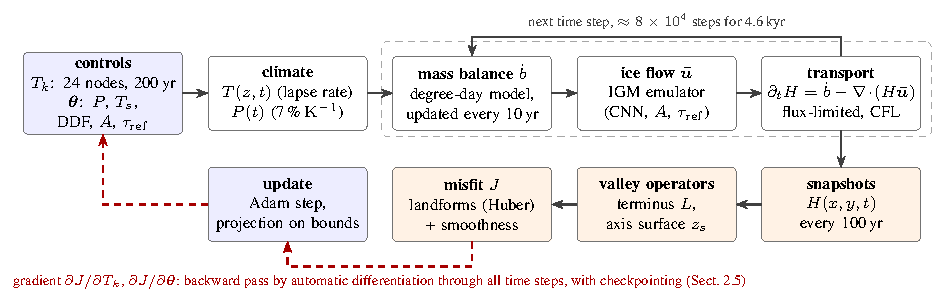
\includegraphics[width=\textwidth]{figures/fig01_schematic.pdf}
\caption{The inversion. A forward run (black arrows) turns the temperature nodes $T_k$ and the parameters $\boldsymbol\theta$ into the ice thickness $H(x,y,t)$, by repeating the mass balance, ice-flow and transport steps (dashed box) over the whole window. Snapshots of $H$ are compared with the dated landforms along the valley flowlines. The gradient of the misfit with respect to all controls is obtained by automatic differentiation (red dashed arrows) and used by the optimiser.}
\label{fig:schematic}
\end{figure*}


\subsection{Ice flow and mass transport}
\label{sec:flow}

The ice thickness $H(x,y,t)$ over the bed $b(x,y)$ evolves by mass conservation,
\begin{equation}
\frac{\partial H}{\partial t} = \dot b - \nabla\cdot\left(H\,\ubar\right),
\label{eq:mass}
\end{equation}
where $\dot b$ is the surface mass balance in metres of ice per year and $\ubar$ the depth-averaged horizontal velocity. We compute $\ubar$ with the ice-flow emulator of the Instructed Glacier Model (IGM), a convolutional neural network that maps the thickness, the surface elevation $s=b+H$, the rate factor $A$ of Glen's flow law, the sliding parameter $\taur$ and the grid spacing to the horizontal velocity at the bed and at the surface \citep{jouvet2022,jouvet2023pinn}. IGM trains its emulators by minimising the energy associated with the higher-order (Blatter--Pattyn) ice-flow equations, so that the network approximates their solution without solving them \citep{jouvet2023pinn}. The architecture that we use (SIADecompNet) adds a learned residual to a basal-sliding and an internal-deformation component of the velocity, through 18 convolutional layers of 80 filters whose dilated kernels see several kilometres around each cell. Basal sliding follows a Weertman law,
\begin{equation}
\tau_b = \taur\left(\frac{|\vec u_b|}{u_\mathrm{ref}}\right)^{1/m},
\label{eq:sliding}
\end{equation}
with $m=3$ and $u_\mathrm{ref}=100$\,\myr, so that a lower $\taur$ means more sliding. The velocity is resolved at two vertical nodes with the mono-layer higher-order basis of \citet{dossantos2022}, and its exact depth average is $\ubar = 0.2\,\vec u_b + 0.8\,\vec u_s$ for a Glen exponent $n=3$. We ported the network and its pretrained weights from TensorFlow to PyTorch, and the port reproduces the original to a relative error of $2.4\times10^{-6}$. The weights are those of the IGM example for the Great Aletsch Glacier, and they were not retrained for the Mont Blanc massif.

Equation~(\ref{eq:mass}) is discretised with finite volumes on the model grid. The fluxes are upwinded on a staggered grid, with a MUSCL reconstruction of the thickness and a superbee slope limiter \citep{vanleer1979,roe1986}. The time step follows the Courant condition, $\Delta t=\min(C\,\Delta x/\max|\ubar|,\ 1\,\mathrm{yr})$ with $C=0.3$, and the depth-averaged speed is capped at 600\,\myr\ to remove the velocity spikes that the emulator produces on single cells of very steep ice, such as the icefall below Lognan. Ice may only grow inside a prescribed area (Sect.~\ref{sec:data}); outside it, a positive mass balance is replaced by $-10$\,\myr.


\subsection{Surface mass balance driven by a temperature history}
\label{sec:smb}

The control is the mean annual air temperature $T(t)$ at a reference elevation $z_\mathrm{ref}=2000$\,m. It is defined at nodes $T_k$ every 200\,yr and interpolated linearly in between. The temperature at the surface elevation $z$ is
\begin{equation}
T(z,t) = T(t) - \Gamma\,(z-z_\mathrm{ref}),
\label{eq:lapse}
\end{equation}
with a lapse rate $\Gamma=7$\,\unit{^{\circ}C\,km^{-1}}, and within the year it follows a cosine of half-range $T_s$,
\begin{equation}
T(z,t,\tau) = T(z,t) - T_s\cos(2\pi\tau),\qquad 0\le\tau<1.
\label{eq:season}
\end{equation}
The fraction of the year below 0\,\degC\ and the positive degree days then have closed forms. With $x=T(z,t)/T_s$,
\begin{equation}
\varphi = \frac{1}{\pi}\arccos x,\qquad
\mathrm{PDD} = N_d\int_0^1 \max\!\left(T(z,t,\tau),0\right)\mathrm{d}\tau = N_d\left[T(z,t)\,(1-\varphi)+\frac{T_s}{\pi}\sqrt{1-x^2}\right],
\label{eq:pdd}
\end{equation}
for $|x|<1$, with $N_d=365.25$\,\unit{d\,yr^{-1}}, while $\mathrm{PDD}=N_d\,T(z,t)$ and $\varphi=0$ when the temperature stays positive all year, and $\mathrm{PDD}=0$ and $\varphi=1$ when it stays negative. To keep the derivatives finite at $|x|=1$, the clipping of $x$ to $[-1,1]$ is replaced by a quadratic blend over $\pm0.1$. All precipitation that falls below 0\,\degC\ is taken as snow, and melt is proportional to the positive degree days, so that the mass balance is
\begin{equation}
\dot b = \frac{\rho_w}{\rho_i}\left[P(t)\,\varphi - f\,\mathrm{PDD}\right],
\label{eq:smb}
\end{equation}
where $f$ is the degree-day factor (in \unit{m\,w.e.\,K^{-1}\,d^{-1}}), $\rho_w/\rho_i=1000/910$ converts water to ice equivalent, and the precipitation $P$ is uniform in space. It follows the temperature at 7\,\% per degree, as expected from the Clausius--Clapeyron relation,
\begin{equation}
P(t) = P_0\,(1+\alpha)^{T(t)-T_\mathrm{p}},\qquad \alpha=0.07\,\unit{K^{-1}},
\label{eq:cc}
\end{equation}
where $P_0$ is the present-day precipitation and $T_\mathrm{p}$ the present-day (2012--2021) temperature at $z_\mathrm{ref}$. We report the result as the anomaly $\Delta T(t)=T(t)-T_\mathrm{p}$. The mass balance is recomputed from the evolving surface every 10\,yr, so that the feedback between surface elevation and mass balance is resolved. This degree-day scheme is deliberately simple \citep{hock2003}. Its parameters $P_0$, $T_s$ and $f$ are calibrated on the present-day glacier (Sect.~\ref{sec:calib}) and are then either held fixed or inverted jointly with $T(t)$ (Sect.~\ref{sec:joint}).


\subsection{From a simulated glacier to dated landforms: valley-referenced operators}
\label{sec:operators}

A dated landform says something about the glacier that built it, not about the ice that happens to lie nearest to it. A first set of operators, which scored the simulated ice at the cells of each landform, failed in two ways. A glacier that stopped short of a moraine scored a constant misfit with no gradient, since there was no ice to move. And ice draped on a valley side or on a nunatak next to a moraine crest was scored as if it were the glacier that built it. We therefore refer every landform to the valley that its ice came down.

For each valley, we trace a flowline down the valley floor, following the steepest descent on the bed after filling its depressions \citep{barnes2014}, from the head of the glacier down past its outermost landform (Fig.~\ref{fig:operators}a). Every cell of a landform is referred to the nearest cell of the flowline, which defines its cross-section on the valley axis. Two quantities of the simulated glacier are measured along the flowline. Both are differentiable and both are defined however far the glacier is from the landform.

The first is the position of the terminus $L$, an arc length along the flowline. It is a soft maximum of the arc lengths $s_i$ of the flowline cells, weighted by a soft indicator of ice and by its continuity with the glacier upstream,
\begin{equation}
L = \tau_L\ln\sum_i w_i\,\mathrm{e}^{s_i/\tau_L},\qquad
w_i = \left(1-\mathrm{e}^{-H_i/H_m}\right)\prod_{j<i}g(H_j),
\label{eq:terminus}
\end{equation}
where $\tau_L=100$\,m sets the smoothness, $H_m=30$\,m, and $g$ is a smoothstep that rises from 0 without ice to 1 at 5\,m of ice. A tongue of another glacier that lies further down the same valley floor is therefore not counted, because the ice between them is missing. The derivative of $L$ only sees the thickness of the snout cell, since the glacier advances on the grid by filling the next cell, an event that the adjoint cannot see. This underestimates the sensitivity of the terminus by a factor of about 50 compared with finite differences. We therefore keep the value of $L$ but take its gradient from the volume of the connected glacier per unit width, $V=\sum_i H_i\,\Delta s_i$, scaled by the change of $V$ per metre of advance, $V_L$, which we measured in constant-temperature runs (690\,m for Argenti\`ere):
\begin{equation}
\tilde L = L + \frac{V-\sg(V)}{V_L},
\label{eq:surrogate}
\end{equation}
where $\sg$ stops the gradient. This straight-through surrogate \citep{bengio2013} has the value of $L$ and the derivative of the volume that feeds an advance.

%f
\begin{figure*}[t]
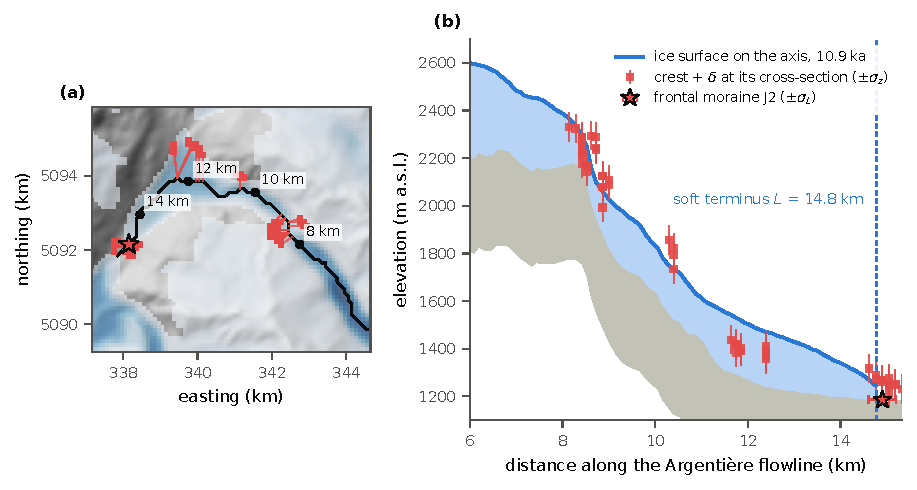
\includegraphics[width=\textwidth]{figures/fig02_operators.pdf}
\caption{Valley-referenced operators on the Argenti\`ere glacier, shown on the jointly inverted glacier at 10.9\,ka. (a) Flowline (black, with distances) and moraine crests (red); thin red lines join crest cells to their cross-sections on the valley axis. Blue shading is the modelled ice thickness. (b) Along the flowline: bed (grey), ice surface on the axis (blue), crest elevations plus the offset $\delta$ at their cross-sections with $\pm\sigma_z$, the frontal moraine J2 with $\pm\sigma_L$, and the soft terminus position $L$ of Eq.~(\ref{eq:terminus}).}
\label{fig:operators}
\end{figure*}

The second quantity is the elevation of the ice surface on the valley axis, $z_s=b+H$, at the cross-section of each landform cell. Each type of landform is then scored as follows (the constraints are listed in Sect.~\ref{sec:data}).
\begin{itemize}
\item A frontal moraine asks that the terminus stood at the moraine, $r=(L-s_\mathrm{obs})/\sigma_L$, at some time within its age window.
\item A lateral moraine asks that the glacier reached its cross-section and that the axis surface stood at the elevation of the crest $z_c$ plus an offset $\delta$, at some time within its age window: $r^2=(\max(0,s_\mathrm{req}-L)/\sigma_L)^2+\langle((z_s-z_c-\delta)/\sigma_z)^2\rangle$, where $\langle\cdot\rangle$ is the mean over the cells of the moraine.
\item A bedrock surface or an erratic boulder asks that the axis surface stayed below the sample elevation $z_r$ plus $\delta$ at all times after its exposure: $r^2=\langle(\max(0,z_s-z_r-\delta)/\sigma_z)^2\rangle$.
\item A dated moraine that survived asks that no later advance overrode it, with the same one-sided form applied after its formation, and a weight of 0.5.
\end{itemize}
The offset $\delta=10$\,m and the uncertainty $\sigma_z=60$\,m are the median and the scatter of the difference between the axis surface and the margin elevation along the Little Ice Age (LIA) Argenti\`ere glacier, mapped by \citet{reinthaler2025}. We use $\sigma_L=300$\,m for a dated frontal moraine. Lateral moraines that are not dated but that \citet{protin2019} assign to the Younger Dryas--Early Holocene transition by morphostratigraphy are used with a weight of 0.5.

The misfit is evaluated on snapshots of $H$ saved every 100\,yr. A moraine was built at one moment within its age window, not at its nominal age, so its misfit is the soft minimum over the snapshots in the window, $S(v_1,\dots,v_n)=-\ln\left(n^{-1}\sum_j \mathrm{e}^{-v_j}\right)$. A bedrock sample and a moraine that survived must hold at all times, so their misfit is the mean over the snapshots. Each landform then counts once in the data term, through a Huber function $h$ that grows linearly beyond $3\sigma$ \citep{huber1964}, so that a single constraint that the model cannot fit does not dominate:
\begin{equation}
D = \sum_g w_g\,h(r_g^2),\qquad h(v)=\begin{cases} v & \text{if } v\le 9,\\ 6\sqrt{v}-9 & \text{otherwise}.\end{cases}
\label{eq:data}
\end{equation}
A constraint that is met contributes zero rather than diluting the others, which happened with a mean over all constraints.


\subsection{Objective and optimisation}
\label{sec:objective}

The objective adds to the data term a penalty on the curvature of the temperature history,
\begin{equation}
J = D + \lambda\sum_k\left(T_{k+1}-2T_k+T_{k-1}\right)^2,
\label{eq:objective}
\end{equation}
with $\lambda=1$\,\unit{K^{-2}}. The penalty acts on the curvature and not on the trend, so that it does not pull the temperature towards a constant. The nodes are also kept inside an envelope of temperatures compiled from independent records of the Lateglacial and Early Holocene, by projecting them on it after every step (Sect.~\ref{sec:calib}). A node that ends on a bound therefore signals a conflict between the landforms and these records.

We minimise $J$ with the Adam optimiser \citep{kingma2015}, which scales each step by the history of the gradient of each control, with a learning rate that decreases along a cosine schedule. When an iterate raises $J$ by more than 5\,\% above the best value, or gives a non-finite gradient, the optimiser returns to the best iterate and halves its step. In the joint inversion (Sect.~\ref{sec:joint}), every control is expressed as a fraction $z\in[0,1]$ of its allowed range, $x=x_\mathrm{lo}+z\,(x_\mathrm{hi}-x_\mathrm{lo})$, with one learning rate for all and no prior on the parameters. Since Adam normalises each step, every control can then move by a similar fraction of its range, and no control is favoured. When the mass-balance parameters change, the present-day temperature $T_\mathrm{p}$ is re-fitted to the observed present-day balance (Sect.~\ref{sec:calib}), and its first-order derivative with respect to these parameters is included in the gradient. The paleotemperature is thus always measured relative to a present-day glacier that has the observed mass balance.


\subsection{Gradients through millennia}
\label{sec:gradients}

The forward model is written in PyTorch \citep{paszke2019}, and the gradient of $J$ with respect to all controls is obtained by reverse-mode automatic differentiation through every time step \citep{baydin2018,griewank2008}. The cost of one gradient is a few forward runs, independently of the number of controls. The difficulty is memory. The backward pass needs the intermediate states of the forward run, and storing the whole computational graph costs about 1\,GB per time step on our 100\,m grid, mostly for the activations of the emulator (Sect.~\ref{sec:cost}). A Lateglacial run of $8\times10^4$ steps would need about 85\,TB. We therefore use checkpointing \citep{griewank2000,chen2016}. Each time step stores only its inputs and recomputes its internal states during the backward pass, which brings the memory down to 0.53\,MB per step, and the run is further divided into blocks of 300 steps whose inputs alone are stored (two-level checkpointing). The memory then grows with $N/300+300$ instead of $N$ for $N$ steps, at the price of one additional forward run. The network and the transport are compiled with \texttt{torch.compile}, which makes a forward and backward pass about 2.8 times faster.

Automatic differentiation computes the exact derivative of the discrete model, but this derivative is not always a useful gradient over thousands of years. We found two instabilities by comparing the adjoint with finite differences (Table~\ref{tab:gradcheck}), and we removed them by differentiating a slightly simpler model than the one we run.
\begin{enumerate}
\item The derivative of the superbee-limited flux is not a stable adjoint. Going backward in time, the sensitivity that it reports grew by a factor of about two every 200\,yr, while finite differences show that the glacier forgets its state within a few centuries. At 11\,ka, it gave the ice surface at Lognan a sensitivity to temperature of $+452$\,\unit{m\,K^{-1}}, of the wrong sign, against $-42$\,\unit{m\,K^{-1}} by finite differences. We therefore run the superbee scheme forward but differentiate a first-order upwind flux, through the straight-through construction $\nabla\cdot\vec q_\mathrm{adj}+\sg(\nabla\cdot\vec q-\nabla\cdot\vec q_\mathrm{adj})$, whose value is that of the superbee flux $\vec q$ and whose derivative is that of the monotone upwind flux $\vec q_\mathrm{adj}$. The sensitivity at Lognan becomes $-39$\,\unit{m\,K^{-1}}, and that of a node 2400\,yr earlier vanishes, as with finite differences.
\item The full adjoint, which differentiates the velocity with respect to the geometry through the emulator, exploded in one Lateglacial iterate, reaching $3\times10^{24}$ in a single cell that held 6\,m of ice, through the feedback between thickness and velocity. We therefore hold the velocity constant within each time step when differentiating (frozen-velocity adjoint). This adjoint stays bounded, halves the cost of the backward pass, and points in the same direction as the full one where both are finite (cosine similarity 0.93). It is about 2.7 times larger, a scale to which Adam is insensitive.
\end{enumerate}
In addition, the time step that the Courant condition sets is treated as a constant in the adjoint, and the gradient of the terminus is taken from Eq.~(\ref{eq:surrogate}). As a safeguard, the adjoint of the thickness is bounded at 0.05 per time step, and non-finite entries are set to zero. This bound was never reached in the temperature-only inversion (largest value 0.016), and only slightly in three of the 30 iterations of the joint inversion (0.057). With these choices, the gradient has the right sign and magnitude for the quantities that matter (Table~\ref{tab:gradcheck}).

The frozen-velocity adjoint gives no derivative with respect to the parameters that act only through the emulator, $A$ and $\taur$. A full-adjoint estimate of their effect on the inferred temperature was moreover about ten times larger than forward runs showed (Sect.~\ref{sec:sensitivity}). In the joint inversion, we therefore compute these two derivatives by one-sided finite differences, with a step of 3\,\% of the allowed range, at the cost of two additional forward runs per iteration.

%t
\begin{table*}[t]
\caption{Gradient check on the Argenti\`ere glacier at 11\,ka (200\,m grid, first mass-balance calibration, constant $T=-1$\,\degC\ at 2000\,m, speed cap 300\,\myr). Sensitivities to a uniform change of temperature, from the adjoint obtained with different choices and from centred finite differences of forward runs.}
\label{tab:gradcheck}
\begin{tabular}{lccc}
\tophline
derivative with respect to $T$ & adjoint of the & upwind adjoint, & finite \\
 & superbee scheme & frozen velocity & differences \\
\middlehline
ice surface at Lognan (\unit{m\,K^{-1}}) & $+452$ & $-39$ & $-42$ \\
terminus position (\unit{m\,K^{-1}}) & $-209$ & $-675^{a}$ & $-968$ \\
temperature node 2400\,yr earlier (\unit{m\,K^{-1}}) & $+201$ & $\approx0$ & $0$ \\
\bottomhline
\end{tabular}
\belowtable{$^{a}$ With the volume surrogate of Eq.~(\ref{eq:surrogate}); without it, the adjoint sees about 1/50 of the finite-difference sensitivity.}
\end{table*}


\subsection{Uncertainty}
\label{sec:uncertainty}

We distinguish the uncertainty that comes from the data and the uncertainty that comes from the fixed parameters. For the first, we shift the nodes of one period uniformly by $u$ and fit a parabola to $J(u)$ through three or four forward runs. Since $J$ is, up to a constant, twice a negative log-likelihood, the curvature gives a data-only standard deviation $\sigma=\sqrt{2/J''}$ for that period. We do this for the Aller\o d (13.6--12.9\,ka), the Younger Dryas (12.9--11.7\,ka), the Preboreal (11.7--10.0\,ka) and the Early Holocene (10.0--9.0\,ka).

For the second, we change one parameter at a time to the bounds of its literature range. If it is a mass-balance parameter, we re-fit $T_\mathrm{p}$ to the present-day balance. We then find, again from a parabola through forward runs, the uniform shift of the whole temperature history that minimises $J$ with the new parameter. A full re-inversion for each parameter would cost about 17\,h, and the uniform shift captures the first-order effect on the mean temperature. The change of the anomaly $\Delta T$ is the sensitivity to that parameter. For the lapse rate and for the scaling of the Lateglacial precipitation, for which we did not run forward models, we use the first-order estimate $\mathrm{d}u^\ast/\mathrm{d}\theta=-J_{u\theta}/J_{uu}$ from the implicit-function theorem, with both derivatives obtained by the adjoint at two values of $u$. The parameter contributions are added in quadrature.


\section{Application to Argenti\`ere glacier and the upper Arve valley}
\label{sec:application}

\subsection{Setting and data}
\label{sec:data}

Argenti\`ere glacier, in the Mont Blanc massif (France), covered about 16\,\unit{km^2} in 2012 and descended from above 3600 to about 1650\,m (Fig.~\ref{fig:map}). It is among the best monitored glaciers of the Alps, with mass-balance measurements since the 1970s and repeated measurements of its thickness and surface \citep{vincent2009,six2014,reveillet2017,rabatel2018,beraud2023}. During the Lateglacial, its tongue descended to La Joux, on the floor of the Arve valley at about 1190\,m, 14.9\,km along its flowline. There, \citet{protin2019} dated a frontal moraine (J2) and an erratic boulder, and they mapped an outer lateral moraine (J1). Upvalley, they dated three lateral moraines at Lognan (L1 to L3) and several bedrock surfaces. \citet{protin2021} dated two lateral moraines (T1 and T2) on the Jardin de Tal\`efre, a bedrock island in the Tal\`efre glacier, which flows into the Mer de Glace. Bedrock exposure ages along the Mer de Glace come from transects at the Aiguille du Moine and the T\^ete de Tr\'elaporte \citep{lehmann2019,lehmann2020}, and from the Remuaz fault scarp and the Cheserys slope above the Arve \citep{cara2017,courtialmanent2023}. We use the ages, their uncertainties and the landform geometries of the AlpIce-1 database \citep{kamleitner2026}, in which all exposure ages are recalculated consistently. Table~\ref{tab:obs} lists the constraints.

%t
\begin{table*}[t]
\caption{Dated landforms used in the inversion. Ages are AlpIce-1 event ages and external 1$\sigma$ uncertainties \citep{kamleitner2026}, converted to ka before 1950\,CE. For the bedrock samples, the constraint applies from the young end of the 1$\sigma$ age onward.}
\label{tab:obs}
\begin{tabular}{p{4.7cm}p{3.1cm}p{4.6cm}p{3.6cm}}
\tophline
landform and site & age (ka) & constraint & source \\
\middlehline
frontal moraine J2, La Joux & $10.84^{+1.07}_{-1.04}$ & terminus at the moraine within the age window ($\sigma_L=300$\,m) & \citet{protin2019} \\
lateral moraines L1, L2, L3, Lognan & $11.59^{+1.10}_{-1.06}$, $10.30^{+0.79}_{-0.78}$, $10.26\pm0.71$ & glacier reaches the cross-section, axis surface at the crest ($\sigma_L=300$\,m, $\sigma_z=60$\,m) & \citet{protin2019} \\
lateral moraines T1, T2, Jardin de Tal\`efre & $11.88\pm0.77$, $11.08\pm0.68$ & as above & \citet{protin2021} \\
lateral moraine J1 and three undated crests, La Joux and Lognan & 13.13--10.83$^{a}$ & as above, weight 0.5 & \citet{protin2019} \\
erratic boulder, La Joux & $13.17\pm0.78$ & no ice above the sample after exposure ($\sigma_z=60$\,m) & \citet{protin2019} \\
bedrock (5 samples), Lognan & 12.49--9.78 & as above & \citet{protin2019} \\
bedrock (1 sample), Jardin de Tal\`efre & $12.36\pm0.73$ & as above & \citet{protin2021} \\
bedrock (7 samples), Aiguille du Moine and T\^ete de Tr\'elaporte & 18.06--11.53 & as above & \citet{lehmann2019,lehmann2020} \\
bedrock (3 samples), Remuaz and Cheserys & 19.09--12.24 & as above & \citet{cara2017}, \citet{courtialmanent2023} \\
survival of the six dated moraines & after formation & no later overriding, weight 0.5 & -- \\
\bottomhline
\end{tabular}
\belowtable{$^{a}$ Morphostratigraphic window: younger than the erratic in front of J1 and older than J2; weight 0.5.}
\end{table*}

%f
\begin{figure*}[t]
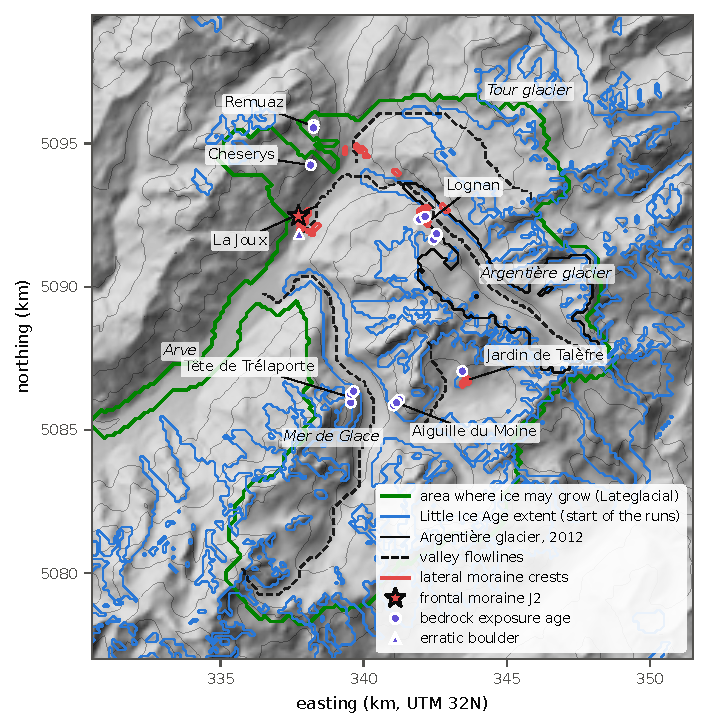
\includegraphics[width=0.86\textwidth]{figures/fig03_study_area.pdf}
\caption{The upper Arve valley and the Lateglacial constraints on the 100\,m model grid. Hillshade of the bed, with 500\,m contours. Ice may grow only inside the green line. The Little Ice Age extent \citep{reinthaler2025} is the initial state of the runs. Red lines are the crests of the dated and mapped lateral moraines, the star is the frontal moraine J2, and purple symbols are bedrock exposure ages and the erratic boulder at La Joux. Dashed lines are the flowlines of the Argenti\`ere, Tal\`efre, Mer de Glace and Tour glaciers. Coordinates are UTM zone 32N.}
\label{fig:map}
\end{figure*}

The model grid covers 25 by 25\,km at 100\,m resolution (250 by 250 cells), including the Argenti\`ere, Tour and Mer de Glace glaciers and the Arve valley floor below La Joux. Ice may grow in an area of 167\,\unit{km^2} that covers the upper Arve basin and the valley floor for 8\,km below the confluence with the Arveyron, so that the tongues never reach the boundary of the domain. The bed is the ice-free topography of \citet{henz2025}, obtained by removing the modelled ice thickness of \citet{cook2023} from a surface elevation model, except under the 2012 Argenti\`ere glacier, where we use the bed measured by radar and blend it over 300\,m. The Argenti\`ere products were 52\,m above the regional elevation model on ice-free terrain, an offset between ellipsoidal and orthometric heights, which we removed before using them. We start the runs at 13.6\,ka from the LIA glacier, whose extent and surface were reconstructed by \citet{reinthaler2025}, because no reconstruction of the Aller\o d glacier exists. The first centuries of the run therefore also act as a spin-up, and the Aller\o d nodes absorb part of the mismatch of this initial state. The window ends at 9.0\,ka, after the last dated constraint. It is 4600\,yr long and takes about $8.3\times10^4$ time steps at 100\,m, with a mean step of about 20\,days.

\subsection{Present-day mass balance}
\label{sec:calib}

The mass balance is calibrated on the 2012--2021 Argenti\`ere glacier. Stake measurements alone do not constrain the temperature and the precipitation separately: they fix the ELA and the mass-balance gradient, and a warmer and wetter climate fits them as well as a colder and drier one. When we fitted the stakes with the temperature at 2000\,m pinned to 1\,\degC, the precipitation had to be 4.7\,\myr, which gives a glacier-wide accumulation of 3.2\,\unit{m\,w.e.\,yr^{-1}}, twice the winter balance of 1.47\,m\,w.e.\ measured with Pl\'eiades images \citep{beraud2023}. We therefore take the precipitation and the seasonality from observations and fit the temperature to the geodetic balance. We use $P_0=1.8$\,\myr, between 1.28\,\myr\ measured at Chamonix (1042\,m) and the higher values of the accumulation area, and $T_s=9.4$\,\degC, the half-range of the monthly temperatures at Chamonix (January $-2.2$\,\degC, July 16.5\,\degC, 1981--2010). The degree-day factor is limited to 10\,\ddfunit, within the range compiled by \citet{hock2003}, and the calibration places it at this bound. The temperature at 2000\,m is then fitted to the 2012--2021 geodetic balance of $-0.66$\,\mwe\ \citep{beraud2023}. This gives $T_\mathrm{p}=-0.89$\,\degC, a glacier-wide accumulation of 1.40\,\mwe\ (1.47 measured) and a root-mean-square misfit of 0.66\,m\,w.e.\ at the stakes, with the ablation zone melting less than measured. The fitted temperature is about 2\,\degC\ below the Chamonix temperature extrapolated with the lapse rate, and it should be read as an effective temperature for this monthly scheme over the glacier. The ELA of the modelled present-day glacier is 2870\,m. Table~\ref{tab:params} lists these values, the ranges used in the joint inversion, and the envelope of Lateglacial temperatures that bounds the nodes (Sect.~\ref{sec:objective}).

%t
\begin{table*}[t]
\caption{Parameters of the model. The literature values are used in the temperature-only inversion; the ranges are the bounds of the joint inversion. The temperature envelope is given as anomalies relative to pre-industrial (1871--1900), with 2012--2021 taken as 2\,\degC\ warmer \citep{begert2018}.}
\label{tab:params}
\begin{tabular}{p{4.8cm}p{3.2cm}p{2.9cm}p{4.6cm}}
\tophline
parameter & literature value & range (joint) & basis \\
\middlehline
present-day precipitation $P_0$ & 1.8\,\myr & 1.0--1.8\,\myr & Chamonix, glacier-wide accumulation \citep{beraud2023} \\
seasonal half-range $T_s$ & 9.4\,\degC & 7.9--10.9\,\degC & Chamonix 1981--2010 \\
degree-day factor $f$ & 10\,\ddfunit & 8--12\,\ddfunit & \citet{hock2003} \\
flow-law factor $A$ & 78\,\Aunit & 52--117\,\Aunit & \citet{cuffey2010}, IGM default \\
sliding stress $\taur$ & 0.215\,MPa & 0.10--0.25\,MPa & IGM default, training range of the emulator \\
present-day temperature $T_\mathrm{p}$ & $-0.89$\,\degC\ at 2000\,m & re-fitted & geodetic balance 2012--2021 \citep{beraud2023} \\
lapse rate $\Gamma$ & 7\,\unit{^{\circ}C\,km^{-1}} & fixed & \\
precipitation scaling $\alpha$ & 7\,\%\,\unit{K^{-1}} & fixed & Clausius--Clapeyron \\
\middlehline
envelope, Aller\o d (13.6--12.9\,ka) & $-4.0$ to $+0.5$\,\degC & & \citet{heiri2015,samartin2012jqs} \\
envelope, Younger Dryas (12.9--11.7\,ka) & $-6.5$ to $-1.0$\,\degC & & \citet{kerschner2008,protin2019} \\
envelope, Preboreal (11.7--10.0\,ka) & $-4.0$ to $+1.0$\,\degC & & \citet{heiri2015,protin2019} \\
envelope, Early Holocene (10.0--9.0\,ka) & $-2.5$ to $+1.5$\,\degC & & \citet{heiri2014,heiri2015} \\
\bottomhline
\end{tabular}
\end{table*}

\subsection{Sequence of inversions}
\label{sec:sequence}

We proceed in four steps, from cheap to expensive. First, forward runs at constant temperature anomalies of $-2$ to $-5$\,\degC\ on a 200\,m grid show that the landforms are best matched near $-4$\,\degC, which we use as a uniform initial guess. Second, a temperature-only inversion on the 200\,m grid (30 iterations, 5.4\,h) reduces $J$ from 35.3 to 25.9 and provides a prior for the 100\,m grid. Third, a temperature-only inversion on the 100\,m grid (30 iterations, 16.8\,h) gives the result of Sect.~\ref{sec:tonly}, whose sensitivity to the fixed parameters we then evaluate (Sect.~\ref{sec:sensitivity}). Fourth, the joint inversion of the temperature and five parameters on the 100\,m grid (30 iterations, 26.8\,h) gives our final result (Sect.~\ref{sec:joint}). The learning rate decreases from 0.1 to 0.01\,\degC\ on the 200\,m grid, from 0.05 to 0.01\,\degC\ on the 100\,m grid, and from 0.03 to 0.005 of the allowed ranges in the joint inversion. All computations ran on one NVIDIA RTX 4090 graphics card with 24\,GB of memory.

\subsection{Temperature-only inversion}
\label{sec:tonly}


With the literature parameters, the inversion converges smoothly (Fig.~\ref{fig:tonly}a): $J$ decreases from 23.66 to 22.74 in 30 iterations, without a rejected step, and no node ends on the bounds of the envelope (Fig.~\ref{fig:tonly}b). The temperature at 2000\,m is $-5.5$\,\degC\ during the Younger Dryas, an anomaly of $-4.65$\,\degC\ relative to 2012--2021 and of $-2.65$\,\degC\ relative to pre-industrial (Fig.~\ref{fig:tonly}c). The coldest node, $-5.65$\,\degC, is at 12.2\,ka, the temperature stays near the Younger Dryas level until 10.4\,ka, and it then rises by about 3\,\degC\ to 9.0\,ka. The data-only uncertainty is smallest during the Younger Dryas (0.22\,\degC), where most landforms are, and largest during the Aller\o d and the Early Holocene (0.97 and 0.81\,\degC), which only a few bedrock samples constrain.

%f
\begin{figure*}[t]
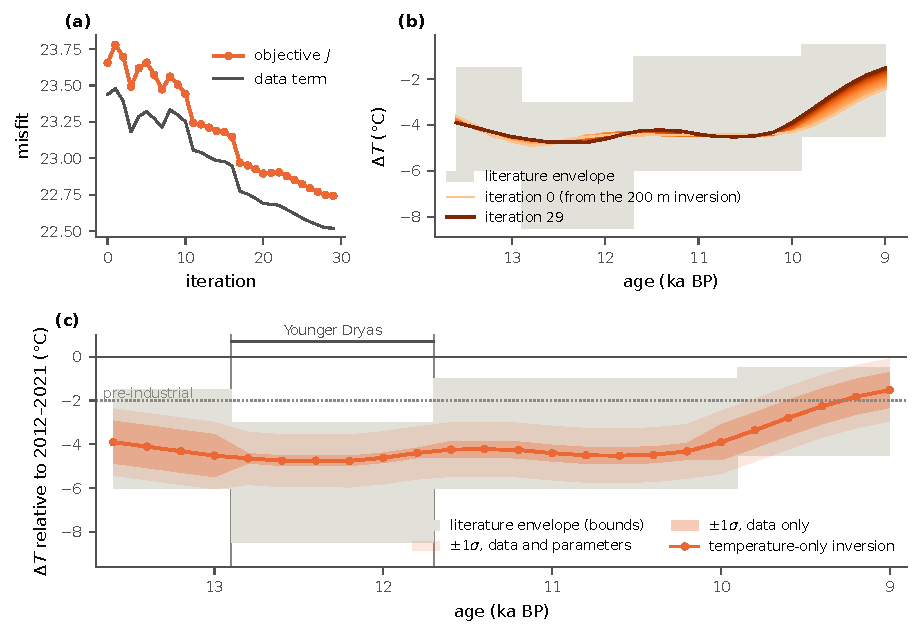
\includegraphics[width=\textwidth]{figures/fig04_temperature_only.pdf}
\caption{Temperature-only inversion on the 100\,m grid, with the literature parameters. (a) Objective $J$ and its data term. (b) Temperature anomaly relative to 2012--2021 at every iteration, starting from the result of the 200\,m inversion; grey is the literature envelope. (c) Final anomaly with its data-only uncertainty and the total uncertainty that includes the fixed parameters (Sect.~\ref{sec:sensitivity}). Vertical lines and the bracket mark the Younger Dryas.}
\label{fig:tonly}
\end{figure*}

The glacier that this temperature history produces reaches the frontal moraine J2 within 129\,m, but only at 11.9\,ka, the old end of its age window. Lognan L2 and the two Tal\`efre moraines are met within $\sigma_z$, and 13 of the 17 bedrock samples remain free of ice after their exposure. The ice surface, however, stands 55 to 80\,m above the lateral moraines at Lognan (L1, L3) and La Joux (J1 and the undated crest), and four bedrock samples are buried under 46 to 149\,m of ice (see also Sect.~\ref{sec:stands}). The modelled glacier is therefore too thick for its length. A colder climate would lengthen it and thicken it further, and a warmer one would thin it but pull its terminus away from J2. The temperature history cannot resolve this conflict, which points to the parameters that set the thickness of the glacier for a given length.

\subsection{Sensitivity to the fixed parameters}
\label{sec:sensitivity}

Figure~\ref{fig:sensitivity} shows how much each fixed parameter moves the Younger Dryas anomaly, and how well the landforms are fitted after the temperature has been shifted to compensate. The parameters of the mass balance move the anomaly but hardly change the fit. A present-day precipitation of 1.5 or 2.1\,\myr\ shifts the anomaly by $-0.55$ and $+0.47$\,\degC, a degree-day factor of 8 or 12\,\ddfunit\ by $+0.33$ and $-0.34$\,\degC, and the seasonality by less than 0.2\,\degC. These parameters trade off with the temperature, both today, through the re-fitted $T_\mathrm{p}$, and in the past. The parameters of the ice flow do the opposite. More sliding ($\taur=0.15$\,MPa) or softer ice ($A=117$\,\Aunit) shift the anomaly by less than 0.08\,\degC, but they reduce the objective from 22.4 to 13.7 and 18.3, because they thin the glacier without shortening it. The largest uncertainty comes from the precipitation during the Lateglacial: if it departed by $\pm25\,\%$ from the Clausius--Clapeyron scaling of the present-day value, the anomaly would change by about $\pm1.0$\,\degC. Combined in quadrature, the parameters contribute $\pm1.17$\,\degC, so that the Younger Dryas anomaly of the temperature-only inversion is $-4.65\pm0.22$ (data) $\pm1.17$ (parameters)\,\degC.

For the ice-flow parameters, the first-order estimate from the full adjoint was ten times or more larger than the forward runs, whereas for the precipitation it agreed to within about 40\,\%. We therefore use forward runs wherever they exist, and treat the two gradient-based contributions (lapse rate and Lateglacial precipitation) as estimates.

%f
\begin{figure*}[t]
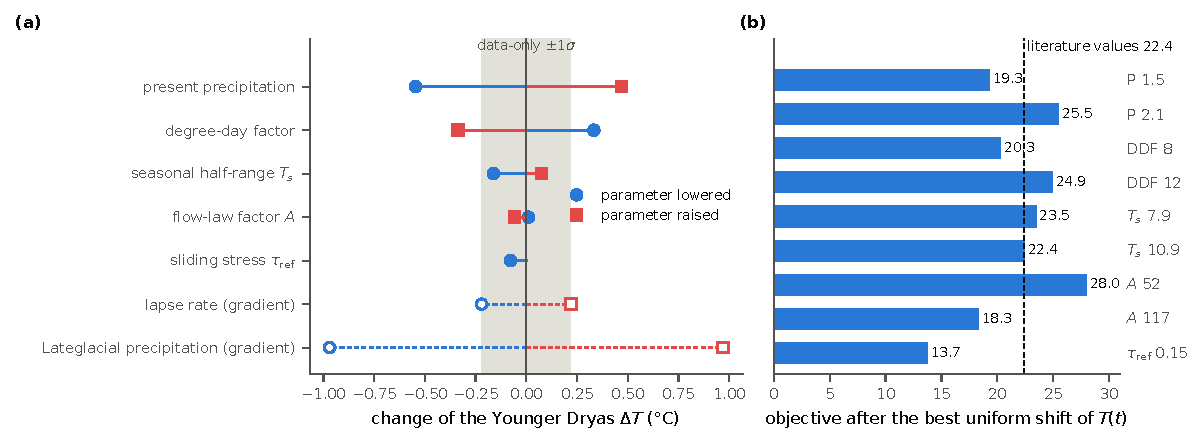
\includegraphics[width=\textwidth]{figures/fig05_sensitivity.pdf}
\caption{Sensitivity of the temperature-only inversion to its fixed parameters. (a) Change of the Younger Dryas anomaly when a parameter is lowered (blue) or raised (red) to the bounds of its range, from forward runs (filled) or from the gradient (open). The mass-balance parameters re-fit the present-day temperature. The grey band is the data-only uncertainty. (b) Objective after the best uniform shift of the temperature history, for each parameter value; the dashed line is the value with the literature parameters.}
\label{fig:sensitivity}
\end{figure*}

\subsection{Joint inversion of temperature and parameters}
\label{sec:joint}

The sensitivity analysis shows that the ice-flow parameters can improve the fit considerably while barely moving the temperature. We therefore invert the 24 temperature nodes jointly with the precipitation $P_0$, the seasonality $T_s$, the degree-day factor $f$, the flow-law factor $A$ and the sliding stress $\taur$, within the ranges of Table~\ref{tab:params}. The inversion starts from the result of the temperature-only inversion and from the literature parameters.

%f
\begin{figure*}[t]
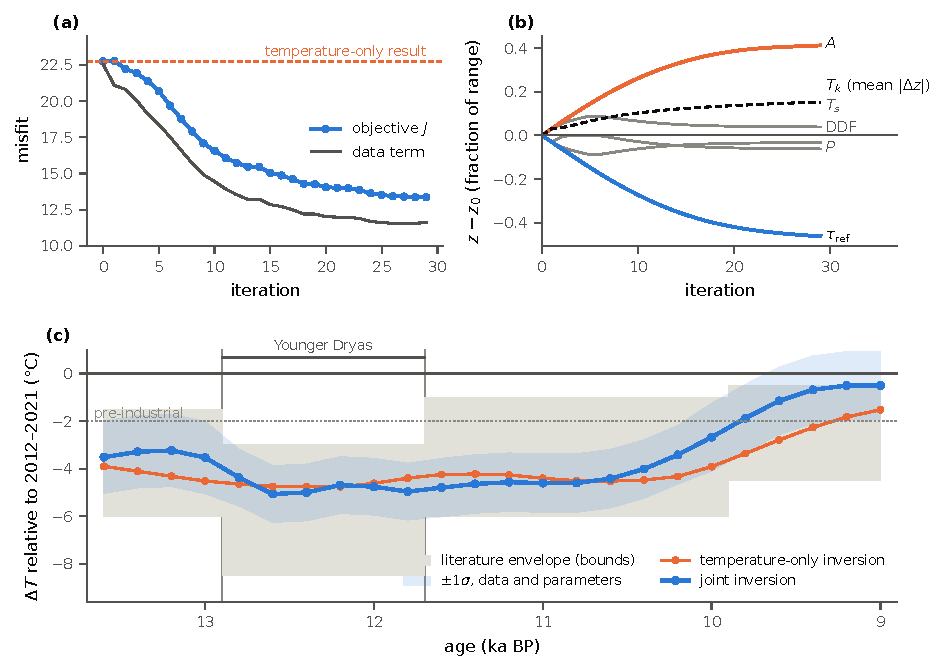
\includegraphics[width=\textwidth]{figures/fig06_joint.pdf}
\caption{Joint inversion of the temperature history and five parameters. (a) Objective $J$ and its data term; the dashed line is the end of the temperature-only inversion. (b) Change of each control since the start, as a fraction of its allowed range; the dashed line is the mean change of the temperature nodes. (c) Temperature anomaly relative to 2012--2021 from the temperature-only (orange) and the joint (blue) inversions, with the total 1$\sigma$ uncertainty of the joint result and the literature envelope (grey).}
\label{fig:joint}
\end{figure*}

The objective decreases from 22.74 to 13.36 (41\,\%), and the data term from 22.52 to 11.60 (Fig.~\ref{fig:joint}a; Table~\ref{tab:results}). The ice-flow parameters move the most (Fig.~\ref{fig:joint}b). The sliding stress decreases from 0.215 to 0.146\,MPa, which means more sliding, and the flow-law factor increases from 78 to 105\,\Aunit, which means softer ice; both move by more than 40\,\% of their ranges. The mass-balance parameters move by 6\,\% of their ranges or less: $P_0=1.75$\,\myr, $T_s=9.52$\,\degC\ and $f=9.87$\,\ddfunit, with a re-fitted $T_\mathrm{p}=-1.00$\,\degC. The present-day glacier is unchanged: its glacier-wide balance is $-0.68$\,\mwe\ ($-0.66$ measured), its accumulation 1.36\,\mwe\ (1.47 measured) and the misfit at the stakes 0.69\,m\,w.e. After 30 iterations, $A$ and $\taur$ were still changing slowly, so the inversion has not fully converged.

The temperature history keeps its shape but gains contrast (Fig.~\ref{fig:joint}c). The Aller\o d is warmer, at $-3.4$\,\degC, the temperature drops by about 1.5\,\degC\ at 12.8\,ka, and the Younger Dryas mean is $-4.81$\,\degC\ relative to 2012--2021 ($-2.8$\,\degC\ relative to pre-industrial). The temperature stays near this level through the Preboreal ($-4.2$\,\degC) until 10.6\,ka, and it then rises by about 4\,\degC\ to $-0.5$\,\degC\ at 9.2\,ka, where the last two nodes reach the warm bound of the envelope. With the uncertainty of Sect.~\ref{sec:sensitivity}, the Younger Dryas anomaly is $-4.8\pm1.2$\,\degC. In the model, it corresponds to a lowering of the ELA by 625\,m, from 2870 to 2245\,m, with the precipitation reduced to 72\,\% of its present value by the Clausius--Clapeyron scaling.

%t
\begin{table}[t]
\caption{Temperature-only and joint inversions on the 100\,m grid. Anomalies are relative to 2012--2021, at 2000\,m. Distances to the landforms are at the best time in the age window (moraines) or the worst time after exposure (bedrock); positive values are ice above the target.}
\label{tab:results}
\begin{tabular}{lcc}
\tophline
 & temperature only & joint \\
\middlehline
objective $J$ (data term) & 22.74 (22.52) & 13.36 (11.60) \\
anomaly, Aller\o d (\degC) & $-4.21$ & $-3.39$ \\
anomaly, Younger Dryas (\degC) & $-4.65$ & $-4.81$ \\
anomaly, Preboreal (\degC) & $-4.32$ & $-4.19$ \\
anomaly, Early Holocene (\degC) & $-2.61$ & $-1.23$ \\
$P_0$ (\myr), $T_s$ (\degC), $f$ (\ddfunit) & 1.80, 9.40, 10.0 & 1.75, 9.52, 9.87 \\
$A$ (\Aunit), $\taur$ (MPa) & 78, 0.215 & 105, 0.146 \\
$T_\mathrm{p}$ (\degC\ at 2000\,m) & $-0.89$ & $-1.00$ \\
terminus minus J2 (m) & $-129$ & $0$ \\
Lognan L1, L2, L3 (m) & $+77$, $+30$, $+62$ & $+48$, $0$, $+7$ \\
La Joux J1, undated crest (m) & $+55$, $+78$ & $+42$, $+73$ \\
Tal\`efre T1, T2 (m) & $+9$, $0$ & $-35$, $-44$ \\
bedrock samples under $>10$\,m of ice & 4 of 17 & 3 of 17 \\
present-day balance, stake misfit (m\,w.e.) & $-0.68$, 0.66 & $-0.68$, 0.69 \\
wall time, 30 iterations & 16.8\,h & 26.8\,h \\
\bottomhline
\end{tabular}
\end{table}

\subsection{The glacier at the dated stands}
\label{sec:stands}

%f
\begin{figure*}[t]
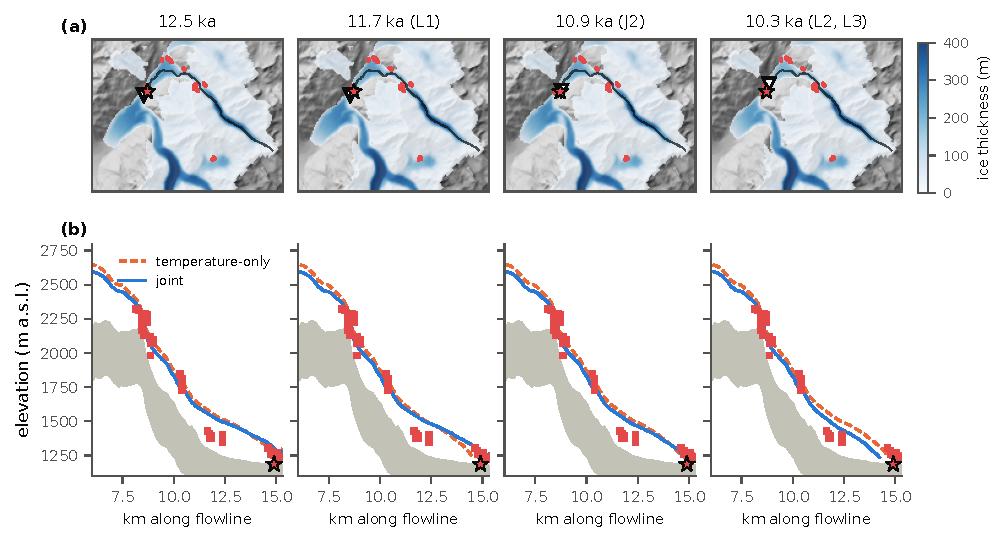
\includegraphics[width=\textwidth]{figures/fig07_stands.pdf}
\caption{The modelled glaciers at four dated stands. (a) Ice thickness of the joint inversion; red lines are moraine crests, the star is J2 and the white triangle the modelled terminus of the Argenti\`ere glacier. (b) Ice surface along the Argenti\`ere flowline for the temperature-only (orange, dashed) and joint (blue) inversions, with the elevations of the lateral moraines at their cross-sections (red squares) and J2 (star).}
\label{fig:stands}
\end{figure*}

The joint inversion produces the same glacier length with a thinner glacier (Fig.~\ref{fig:stands}). At the dated stands, the ice surface along the Argenti\`ere flowline is lower than in the temperature-only inversion, by about 40\,m on average and by 20 to 50\,m along the lower tongue, because faster ice flow carries the ice further for the same thickness. The terminus now stands exactly at J2 at 11.4\,ka, the moraines L2 and L3 are met within 7\,m, and L1 is 48\,m too high instead of 77\,m (Fig.~\ref{fig:fits} and Table~\ref{tab:results}). The gain comes mostly from the bedrock samples. The bedrock at Lognan is now free of ice after its exposure, and only three samples remain covered by more than 10\,m of ice: at the T\^ete de Tr\'elaporte (87\,m), the erratic at La Joux (48\,m) and at the Aiguille du Moine (27\,m). The thinner glacier is now 35 to 44\,m below the Tal\`efre moraines, which slightly worsens their fit, and the lateral crests at La Joux remain 42 to 73\,m too low for the modelled surface.

%f
\begin{figure*}[t]
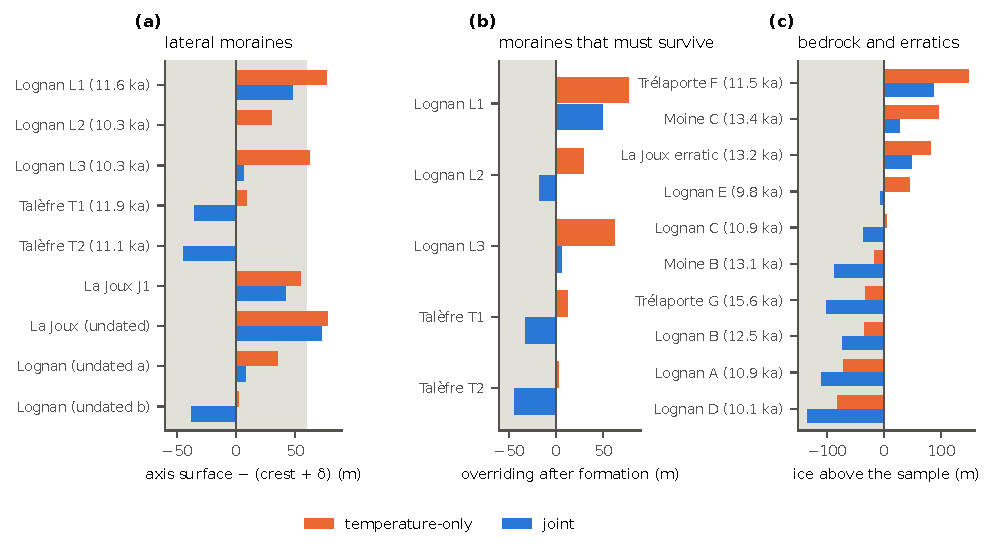
\includegraphics[width=\textwidth]{figures/fig08_landform_fit.pdf}
\caption{Distance of the modelled glaciers to each constraint, for the temperature-only (orange) and joint (blue) inversions. (a) Lateral moraines: axis surface minus crest elevation plus $\delta$, at the best time within the age window; the grey band is $\pm\sigma_z$. (b) Dated moraines that must survive: largest overriding after their formation. (c) The ten bedrock and erratic samples closest to the ice: largest ice thickness above the sample after its exposure. In (b) and (c), the grey band marks the values that satisfy the constraint.}
\label{fig:fits}
\end{figure*}

The terminus of Argenti\`ere glacier advances during the first millennium of the run and reaches La Joux by 12.7\,ka, where it builds the lateral moraine J1 slightly beyond J2 (Fig.~\ref{fig:terminus}). It stays within 0.5\,km of J2 until 10.7\,ka, with a short readvance at 11.9 to 11.5\,ka, and it then retreats by 3.4\,km by 9.0\,ka. This retreat starts about 0.5\,kyr earlier and is faster than in the temperature-only inversion, as the Early Holocene is warmer. The modelled glaciers of the upper Arve covered 156\,\unit{km^2} and held 11.2\,\unit{km^3} of ice at 12.5\,ka, and 114\,\unit{km^2} and 6.1\,\unit{km^3} at 9.0\,ka.

%f
\begin{figure}[t]
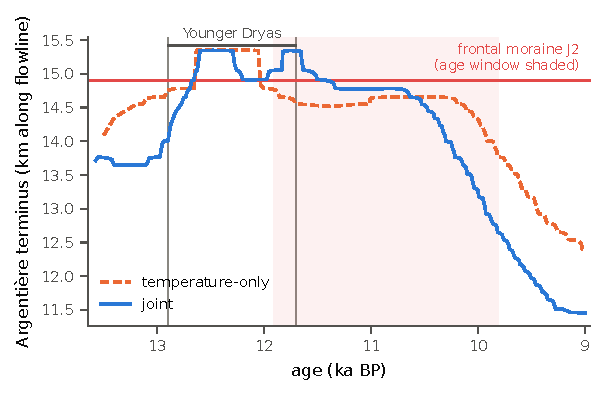
\includegraphics[width=0.62\textwidth]{figures/fig09_terminus.pdf}
\caption{Terminus position of Argenti\`ere glacier along its flowline in the temperature-only (orange) and joint (blue) inversions. The red line is the frontal moraine J2 and the red shading its age window; the bracket marks the Younger Dryas. A terminus at 15.3\,km has reached the end of the flowline, beyond J2.}
\label{fig:terminus}
\end{figure}


\section{Discussion}
\label{sec:discussion}

\subsection{What dated landforms constrain}
\label{sec:constrain}

The two inversions show what the landforms of Argenti\`ere can and cannot tell. A frontal moraine constrains the length of the glacier at some time within its age window, and a lateral moraine or a bedrock sample constrains its thickness. A change of temperature moves both together: a colder climate makes a glacier that is both longer and thicker. A change of ice flow moves them separately: faster flow makes a glacier longer for the same volume, or thinner for the same length. When the temperature alone is inverted, the glacier is long enough but too thick (Sect.~\ref{sec:tonly}), and only a change of ice flow can resolve the conflict. This is why the joint inversion moves $A$ and $\taur$ and not the mass-balance parameters (Fig.~\ref{fig:joint}b), and why the Younger Dryas temperature changes by only 0.16\,\degC\ while the fit improves by 41\,\%.

The mass-balance parameters, in contrast, are not constrained by the landforms. The precipitation, the seasonality and the degree-day factor trade off with the temperature, both today and in the past, and the joint inversion leaves them near their starting values. The landforms constrain the mass balance of the glacier, not the climate that produced it, as for the ELA \citep{ohmura1992}. The temperature that we infer is therefore conditional on these parameters, and they dominate its uncertainty (Fig.~\ref{fig:sensitivity}). This also holds for the precipitation during the Lateglacial, which we tie to the temperature by the Clausius--Clapeyron relation. The landforms cannot test this assumption, and an independent estimate of either the temperature or the precipitation would fix a point on the trade-off, as in ELA-based approaches \citep{kerschner2000,rea2020}.

The data-only uncertainty also shows which periods the landforms constrain. It is 0.22\,\degC\ for the Younger Dryas, where most moraines and bedrock samples are, 0.37\,\degC\ for the Preboreal, and 0.8 to 1.0\,\degC\ for the Aller\o d and the Early Holocene. The Aller\o d is constrained only by bedrock that became free of ice, and it also absorbs the initial state of the run. The Early Holocene is constrained by bedrock at Lognan and by the requirement that the dated moraines survived, and both only bound the temperature from one side. That the last two nodes reach the warm bound of the envelope reflects this: the landforms ask for a smaller glacier, and nothing in the data limits how small.

\subsection{Comparison with independent estimates}
\label{sec:comparison}

Our Younger Dryas anomaly, $-4.8\pm1.2$\,\degC\ relative to 2012--2021, can be compared with the estimates of \citet{protin2019} for the same glacier. With a degree-day model they found temperatures 3.6 to 5.5\,\degC\ lower than in 1979--2002 for the Younger Dryas--Early Holocene transition, and with the rise of the ELA 3.0 to 4.8\,\degC\ lower than in 2008. The Swiss Alps warmed by roughly 1\,\degC\ between 1979--2002 and 2012--2021 \citep[e.g.][]{begert2018}, so that our anomaly corresponds to about $-3.8$\,\degC\ relative to their reference period, within their range. The difference is that their estimates assume a glacier in equilibrium with each moraine, whereas ours accounts for the time that the glacier needs to respond, and that we use all landforms of the valley at once.

The structure of our temperature history can be compared with chironomid-based reconstructions of summer temperature in the Alps. In the southern Swiss Alps, \citet{samartin2012jqs} found a cooling of about 2\,\degC\ at the transition from the Aller\o d to the Younger Dryas and a warming of about 4\,\degC\ at its end, and other Alpine records show changes of similar size \citep{ilyashuk2009,heiri2014,heiri2015}. The joint inversion gives a cooling of about 1.5\,\degC\ at 12.8\,ka and a warming of about 4\,\degC\ between 10.6 and 9.2\,ka. The size of these changes agrees with the chironomids. Their timing differs: in our inversion, the glacier stays near its Younger Dryas extent until about 10.6\,ka, consistent with the moraines dated by \citet{protin2019} at 10.3\,ka, and the warming follows later than the end of the Younger Dryas at 11.7\,ka. Glaciers respond to the mass balance over decades to centuries, and their moraines record the time at which they stood, not the time of the climate change. Moraines of the transition between the Younger Dryas and the Early Holocene are found in several Alpine valleys, which suggests that the deglaciation was interrupted by cold phases \citep{schindelwig2012,moran2016,boxleitner2019,protin2021}. Part of the delay also reflects how the inversion uses the age windows: it matches J2 at 11.4\,ka, but L2 and L3 near the young ends of their 1$\sigma$ windows, at 9.9 and 9.6\,ka. With age uncertainties of 0.7 to 1.1\,kyr for these moraines, and no moraine between 10 and 9\,ka, the timing of the warming is less certain than its size. Note also that the chironomids record the July temperature near lakes, whereas our temperature is an annual mean with a fixed seasonality, at the elevation of the glacier.

The precipitation is the least constrained part of our climate. The Clausius--Clapeyron scaling gives a Younger Dryas precipitation of 72\,\% of the present one. Reconstructions from palaeoglaciers suggest that the western Alps were relatively dry during the Younger Dryas \citep{baroni2021} and that the atmospheric circulation over Europe changed \citep{rea2020}, so that the Lateglacial precipitation may have departed from this scaling. A precipitation 25\,\% lower or higher than our scaling would change the Younger Dryas anomaly by about $\mp1$\,\degC\ (Fig.~\ref{fig:sensitivity}), which is the largest single term of our uncertainty.

\subsection{Choices and limitations}
\label{sec:limitations}

The parameters of the joint inversion are effective, and they also absorb model errors. With $A=105$\,\Aunit, the ice is 1.4 times softer than recommended for temperate ice \citep{cuffey2010}, and the sliding stress of 0.146\,MPa lies within the training range of the emulator, but both may also compensate for the coarse representation of narrow valleys and icefalls at 100\,m, for the speed cap of 600\,\myr, or for an emulator trained on another glacier. Retraining the emulator on the Mont Blanc massif, as IGM allows during an inversion \citep{jouvet2023inv}, would remove this last source of error. The degree-day scheme ignores refreezing, radiation and debris cover. The Mer de Glace tongue is debris covered today, and a debris-free model needs a colder climate to keep it long. In the Lateglacial window, the Mer de Glace is constrained only by bedrock samples, which bound its thickness from above, so that this bias does not enter directly. Thin ice that the model accumulates on steep headwalls, which the real glacier sheds by avalanches, is not observed by the operators along the valley axes.

The landform operators involve choices that set the weight of each constraint: the offset $\delta$ and the uncertainty $\sigma_z$ come from the LIA glacier, the uncertainty of the terminus from the width of a frontal moraine, and the soft minimum over the age window allows each moraine to form at its best time within its 1$\sigma$ age. A moraine dated with an age uncertainty of 1\,kyr can thus be built by a glacier that stands there for a short time anywhere within 2\,kyr, which reduces the information on the timing. A probabilistic treatment of the ages, or a stratigraphic ordering of the moraines, would sharpen it.

The inversion starts from the LIA glacier at 13.6\,ka, and the lapse rate and seasonality are constant in time. The lapse rate could be added to the controls at no extra cost for the gradient, but the landforms cannot distinguish it from the temperature, as for the other mass-balance parameters. Finally, the joint inversion had not fully converged after 30 iterations, and $A$ and $\taur$ were still drifting slowly. Since the Younger Dryas anomaly no longer changed after 20 iterations ($-4.81$\,\degC\ from iteration 20 onward), we do not expect it to change much with more iterations.

\subsection{Cost and scalability}
\label{sec:cost}

%f
\begin{figure}[t]
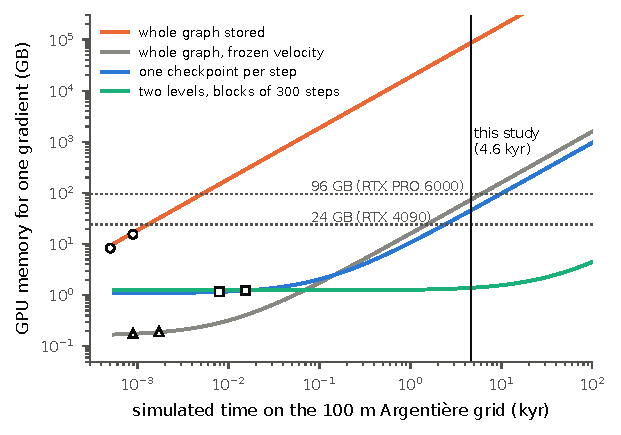
\includegraphics[width=0.62\textwidth]{figures/fig10_memory.pdf}
\caption{GPU memory needed to compute one gradient on the 100\,m Argenti\`ere grid, as a function of the simulated time, for four ways of storing the computational graph. Symbols are measurements over a few hundred time steps; lines extrapolate them linearly in the number of steps (about 18\,000 per kyr). Horizontal lines mark the memory of an RTX 4090 and of an RTX PRO 6000 graphics card.}
\label{fig:memory}
\end{figure}

%t
\begin{table}[t]
\caption{Computational cost on one NVIDIA RTX 4090 (24\,GB). Memory for the 4.6\,kyr window at 100\,m is extrapolated from the measurements of Fig.~\ref{fig:memory}.}
\label{tab:cost}
\begin{tabular}{lc}
\tophline
forward run, 4.6\,kyr at 100\,m ($8.3\times10^4$ steps) & 9\,min \\
gradient, frozen-velocity adjoint, two-level checkpoints & 34\,min \\
gradient, full adjoint & 2.1\,h \\
iteration of the joint inversion (gradient and 2 forward runs) & 54\,min \\
gradient by finite differences (30 controls) & $\approx4.6$\,h \\
memory, whole graph stored & $\approx85$\,TB \\
memory, one checkpoint per step & $\approx45$\,GB \\
memory, two-level checkpoints (blocks of 300 steps) & $\approx1.4$\,GB \\
\bottomhline
\end{tabular}
\end{table}

One gradient of the temperature-only inversion costs 34\,min, about 3.6 forward runs, for 24 controls (Table~\ref{tab:cost}). One-sided finite differences would need 25 forward runs, about 4\,h, and the cost of an ensemble grows even faster: five values for each of the 29 controls of the joint inversion would need $5^{29}\approx2\times10^{20}$ forward runs. The whole inversion sequence of Sect.~\ref{sec:sequence}, from the scans to the joint inversion, took less than three days on one graphics card. The same code inverted a 517\,yr temperature history of the Great Aletsch Glacier from six dated extents in a twin experiment, at 3\,min per iteration (Appendix~\ref{app:twin}). The method is thus not tied to a time scale: it works for centennial histories constrained by mapped extents and for millennial histories constrained by moraines and exposure ages.

The cost of a forward run grows with the number of cells and of time steps, and the number of time steps grows with the length of the period and the speed of the ice, and inversely with the grid spacing. Halving the grid spacing therefore multiplies the cost by about eight, and doubling the period by two. The memory grows in the same way (Fig.~\ref{fig:memory}). Storing the whole graph is possible only for a few dozen time steps. With one checkpoint per step, the 4.6\,kyr window at 100\,m needs about 45\,GB, which exceeds a 24\,GB card but fits on a card with 96\,GB, such as the RTX PRO 6000. With two-level checkpointing, it needs about 1.4\,GB, and a window of 100\,kyr would still fit on a 24\,GB card. More levels, or the binomial checkpointing of \citet{griewank2000}, make the memory grow only logarithmically with the number of steps, at the price of more recomputation. Memory is therefore not a hard limit, but a trade-off with computing time, which a larger card shifts: with 96\,GB, the 4.6\,kyr window can be differentiated without the second level of checkpointing, which saves one forward run per gradient.

Computing time is then the limit. A gradient costs a fixed number of forward runs, so that the time of an inversion is that of a few hundred forward runs, whatever the number of unknowns. Several choices keep this number small. The frozen-velocity adjoint halves the backward pass, compiling the network and the transport makes it about three times faster, and finite differences are used only for the two parameters whose adjoint was unreliable. A coarse-to-fine sequence, as here from 200 to 100\,m, provides a good start for the expensive grid, and the inverse problem can be split into windows that each end at the last observation that they contain. For larger domains, such as the whole Alps during the Last Glacial Maximum, IGM already runs the emulator and the transport on grids of millions of cells on one card \citep[e.g.][]{leger2025}, and the domain can be split across several cards. We see no obstacle of principle to applying the method to other glaciers, ice caps and periods, wherever a bed topography and dated landforms exist.


\conclusions
\label{sec:conclusions}

We have presented a method that infers a temperature history directly from dated glacial landforms, using a differentiable glacier evolution model. The model couples a degree-day mass balance, the ice-flow emulator of IGM and mass transport, and automatic differentiation provides the gradient of the misfit with respect to all temperature nodes and parameters at the cost of a few forward runs. Valley-referenced operators make frontal and lateral moraines and exposure ages differentiable, including when the simulated glacier is far from them. Checkpointing makes millennial runs on a 100\,m grid fit on one graphics card, and two modifications of the adjoint, an upwind transport and a frozen velocity, keep the gradient stable over thousands of years.

At Argenti\`ere and in the upper Arve valley, a temperature-only inversion reproduces the length of the Lateglacial glacier but not its thickness. A joint inversion of the temperature and five parameters resolves this conflict through faster ice flow, reduces the misfit by 41\,\%, and gives a Younger Dryas temperature $4.8\pm1.2$\,\degC\ below that of 2012--2021, followed by a warming of about 4\,\degC\ between 10.6 and 9.2\,ka. The landforms constrain the mass balance of the glacier rather than the climate itself, so that the uncertainty is dominated by the precipitation and the other mass-balance parameters, and an independent estimate of the precipitation would reduce it the most.

The method is general. It needs a bed topography, a mass-balance model and dated landforms, and it applies to any glacier, period and spatial scale. Long simulations and large domains are challenging, because the memory and the computing time grow with the number of cells and of time steps. This growth can be absorbed: checkpointing turns memory into recomputation, simplified adjoints and compiled code reduce the cost of each gradient, a coarse-to-fine sequence reduces the number of expensive iterations, and graphics cards with up to 96\,GB of memory remove most of the recomputation. The next steps are to retrain the emulator during the inversion, to add independent constraints on precipitation, and to apply the method to the full Lateglacial and Holocene record of the Alps compiled in AlpIce-1.


\codedataavailability{The code of the differentiable glacier evolution model, the inversion scripts and the scripts that produce the figures will be archived on Zenodo upon publication (DOI to be added). IGM is available at \url{https://github.com/instructed-glacier-model/igm}. The exposure ages and landform geometries are from AlpIce-1 \citep{alpice2026data}, the LIA extents and surfaces from \citet{reinthaler2024data}, and the bed topography from \citet{henz2025data}. The stake measurements of Argenti\`ere glacier are from the GLACIOCLIM observatory (\url{https://glacioclim.osug.fr}); the 2012 and 2021 thickness and bed products of Argenti\`ere glacier were provided by [to be completed].}

\appendix

\section{Twin experiment on the Great Aletsch Glacier}
\label{app:twin}

To test whether the inversion recovers a known temperature history, we generated synthetic observations with the model and inverted them. The setting is the Great Aletsch Glacier on a 100\,m grid (225 by 132 cells), from 1500 to 2017, starting from the 2017 geometry. The true temperature at the lowest point of the grid stays near 7.2\,\degC\ until about 1800 and then rises along a smooth curve to 8.56\,\degC\ in 2017 (Fig.~\ref{fig:twin}a). It is applied in steps of 10\,yr, and the ice thickness of the true run is saved in 1750, 1880, 1926, 1957, 1980 and 2017. The inversion only sees the extent of the ice at these dates, compared through a soft indicator of ice (1\,m threshold, 5\,m width), and it controls 11 nodes held constant over 50\,yr, with a small penalty on their differences. The other parameters are the same in the true run and in the inversion (degree-day factor 7.4\,\ddfunit, precipitation 1.8\,\myr, $T_s=10$\,\degC, $\taur=0.215$\,MPa, $A=78$\,\Aunit), so that the experiment tests the information in the extents, not the effect of wrong parameters.

%f
\begin{figure*}[t]
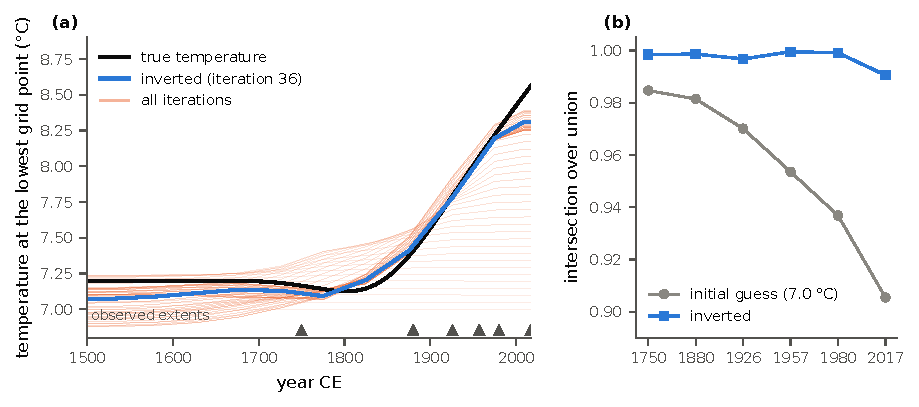
\includegraphics[width=\textwidth]{figures/figA1_twin.pdf}
\caption{Twin experiment on the Great Aletsch Glacier, 1500--2017. (a) True temperature at the lowest grid point (black) and inverted temperature at the best iteration (blue), with all iterations (orange, from light to dark); triangles mark the dates of the observed extents. (b) Intersection over union between the simulated and the true extents at the observation dates, for the initial guess and the inverted temperature.}
\label{fig:twin}
\end{figure*}

Starting from a uniform 7.0\,\degC, the inversion reaches its lowest misfit after 36 iterations of about 3\,min each (Fig.~\ref{fig:twin}). This misfit is lower than that of the true temperature history, so that the remaining differences are not resolved by the extents. The intersection over union between the simulated and the true extents rises from 0.91--0.99 to 0.99--1.00, and the volume is recovered within 1\,\% at all dates but 2017 (3.5\,\%), although only the extent is fitted. Over the observed period, the inverted temperature differs from the truth by 0.07\,\degC\ (root mean square), and the warming from 1500--1749 to 2017 is recovered to 88\,\% (1.20 against 1.36\,\degC). The largest error is in 2017 ($-0.25$\,\degC), at the end of the window, where the last node is constrained by only one extent and the glacier has had no time to respond.


\noappendix

\authorcontribution{KL designed the method, wrote the code, carried out the inversions and wrote the manuscript. (Contributions of the co-authors to be added.)}

\competinginterests{The author declares that there are no competing interests.}

\begin{acknowledgements}
We thank the GLACIOCLIM observatory for the mass-balance data of Argenti\`ere glacier, the providers of the thickness and bed products (to be completed), and the authors of AlpIce-1, of the LIA reconstruction and of the Alps-wide bed topography for making their data available. (Funding and computing resources to be added.)
\end{acknowledgements}


\bibliographystyle{copernicus}
\bibliography{references}

\end{document}
